\documentclass[tikz,border=10pt]{standalone}
\usepackage{tikz}
\usetikzlibrary{shapes.geometric, arrows.meta, positioning}

\begin{document}
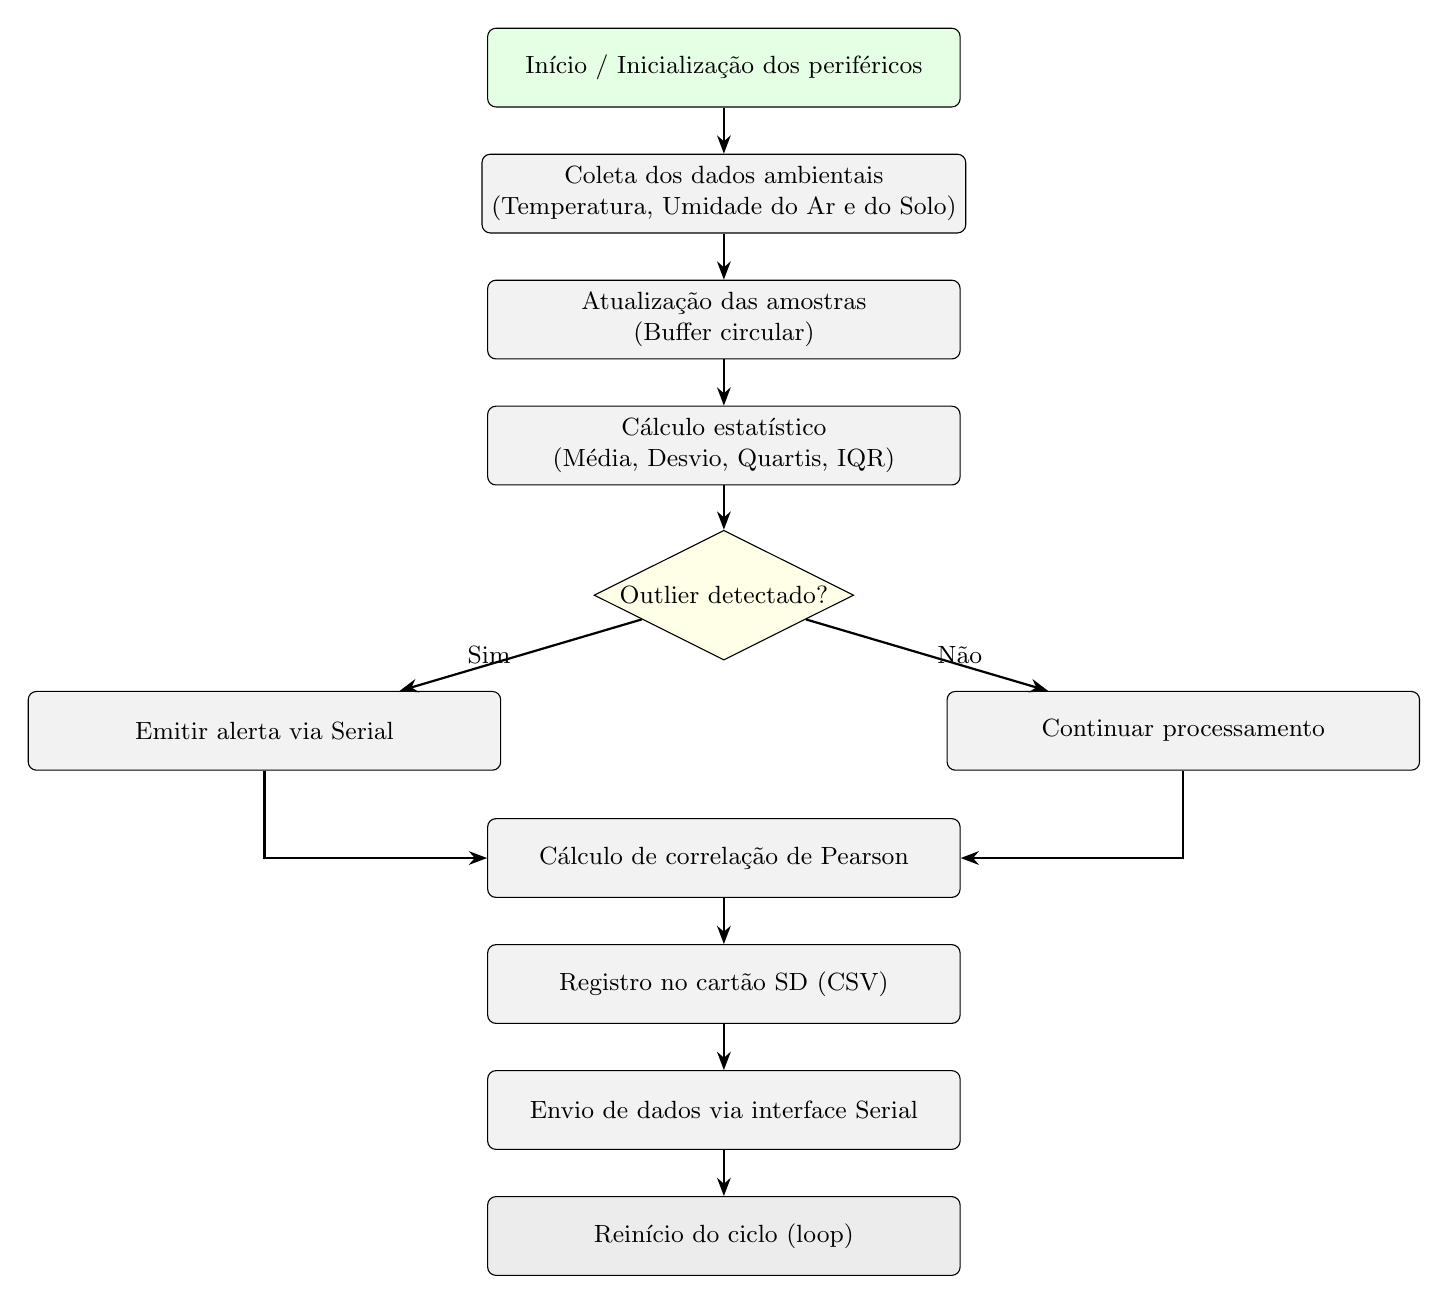
\begin{tikzpicture}[
    node distance=1.6cm,
    every node/.style={font=\small, align=center},
    box/.style={rectangle, draw=black, rounded corners=3pt, minimum width=6cm, minimum height=1cm, fill=gray!10},
    decision/.style={diamond, draw=black, aspect=2, text centered, fill=yellow!10, inner sep=1pt},
    arrow/.style={-Stealth, thick}
]

% NODES
\node[box, fill=green!10] (start) {Início / Inicialização dos periféricos};
\node[box, below of=start] (collect) {Coleta dos dados ambientais\\(Temperatura, Umidade do Ar e do Solo)};
\node[box, below of=collect] (update) {Atualização das amostras\\(Buffer circular)};
\node[box, below of=update] (stats) {Cálculo estatístico\\(Média, Desvio, Quartis, IQR)};
\node[decision, below of=stats, yshift=-0.3cm] (outlier) {Outlier detectado?};
\node[box, below left=0.8cm and 2cm of outlier] (alert) {Emitir alerta via Serial};
\node[box, below right=0.8cm and 2cm of outlier] (normal) {Continuar processamento};
\node[box, below=2cm of outlier] (correlation) {Cálculo de correlação de Pearson};
\node[box, below of=correlation] (save) {Registro no cartão SD (CSV)};
\node[box, below of=save] (serial) {Envio de dados via interface Serial};
\node[box, below of=serial, fill=gray!15] (loop) {Reinício do ciclo (loop)};

% ARROWS
\draw[arrow] (start) -- (collect);
\draw[arrow] (collect) -- (update);
\draw[arrow] (update) -- (stats);
\draw[arrow] (stats) -- (outlier);
\draw[arrow] (outlier) -- node[left]{Sim} (alert);
\draw[arrow] (outlier) -- node[right]{Não} (normal);
\draw[arrow] (alert) |- (correlation);
\draw[arrow] (normal) |- (correlation);
\draw[arrow] (correlation) -- (save);
\draw[arrow] (save) -- (serial);
\draw[arrow] (serial) -- (loop);

\end{tikzpicture}
\end{document}

